\documentclass[../../Problems]{subfiles}
\begin{document}
\subsection{Simpson's Rule}{\label{pp:simpsonsrule}}
{\small% \begin{wrapfigure}{R}{0.1\linewidth}
%   \begin{center}
%   	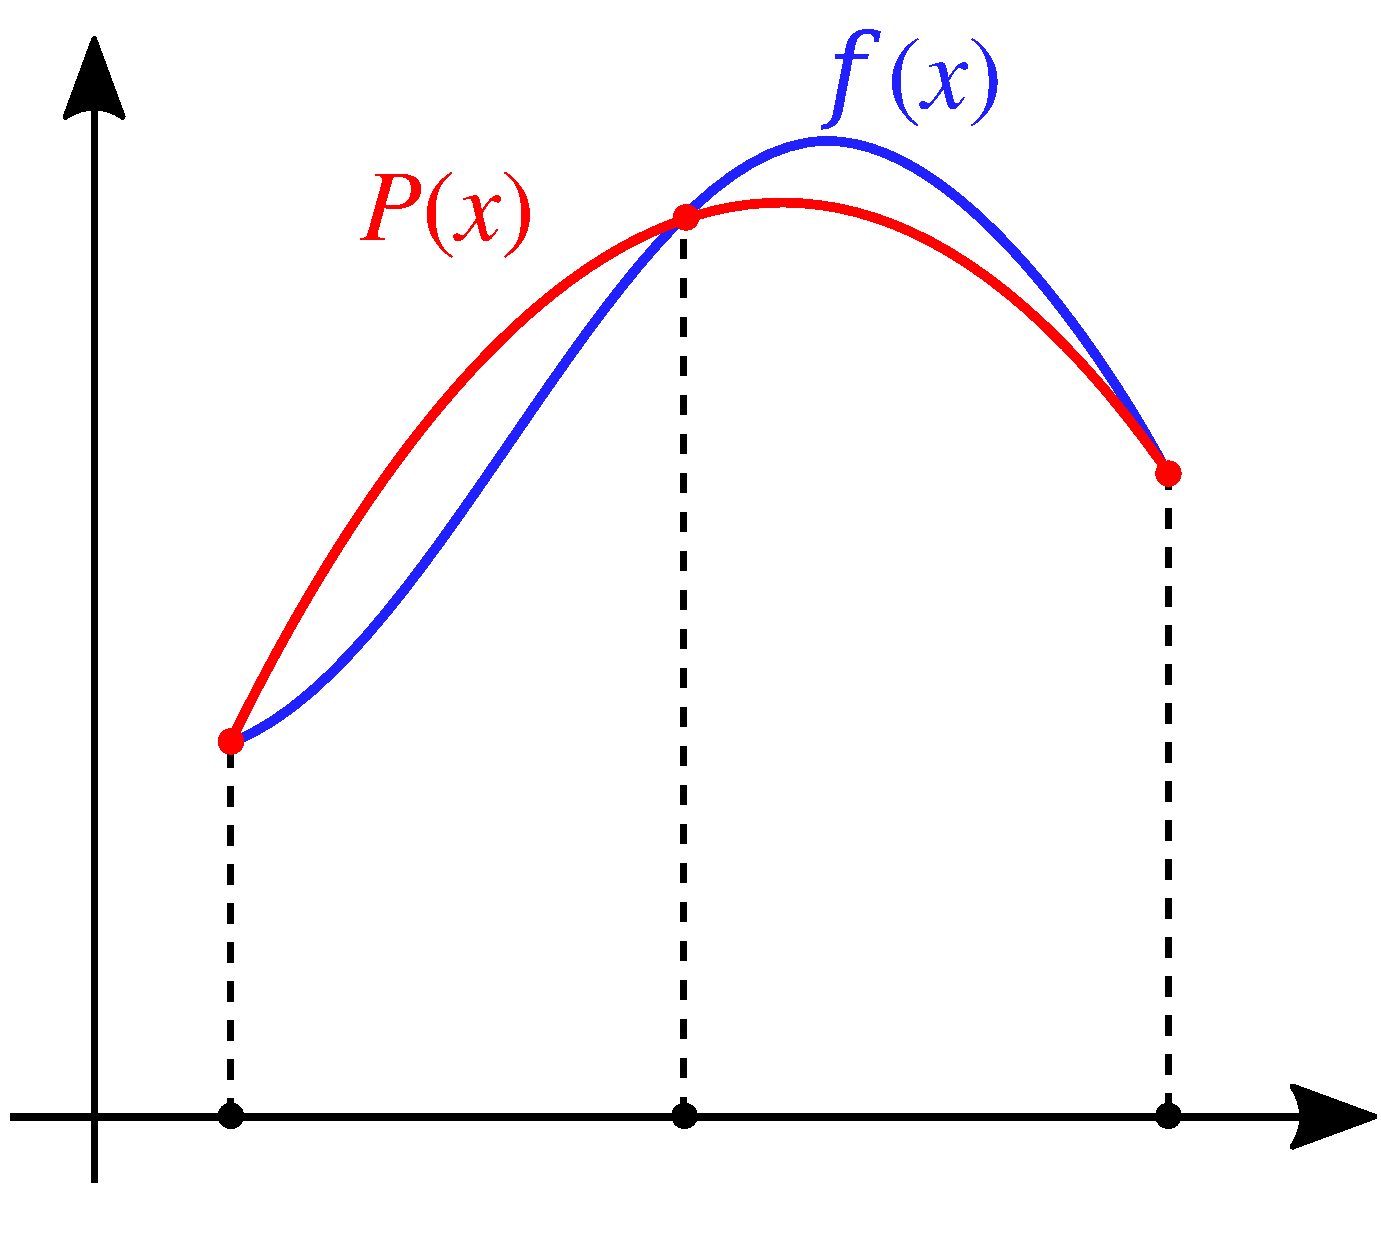
\includegraphics[width = \linewidth]{Simpson's Rule.pdf}
%   \end{center}
%   \caption{}
%   \label{fig:simpsonsrule}
% \end{wrapfigure}
Simpson's Rule is a method in numerical integration (approximating definite integrals).\\
It approximates the area of $f(x)$ in the interval $[a,b]$ by area of parabola passing through $a, \mfrac{a+b}{2}, b$. as shown in \ref{fig:simpsonsrule}.%\footnote{\href{https://bit.ly/simpsonsrule}{Image source}}.%\ref{fig:simpsonsrule}
\begin{figure}[H]
\centering
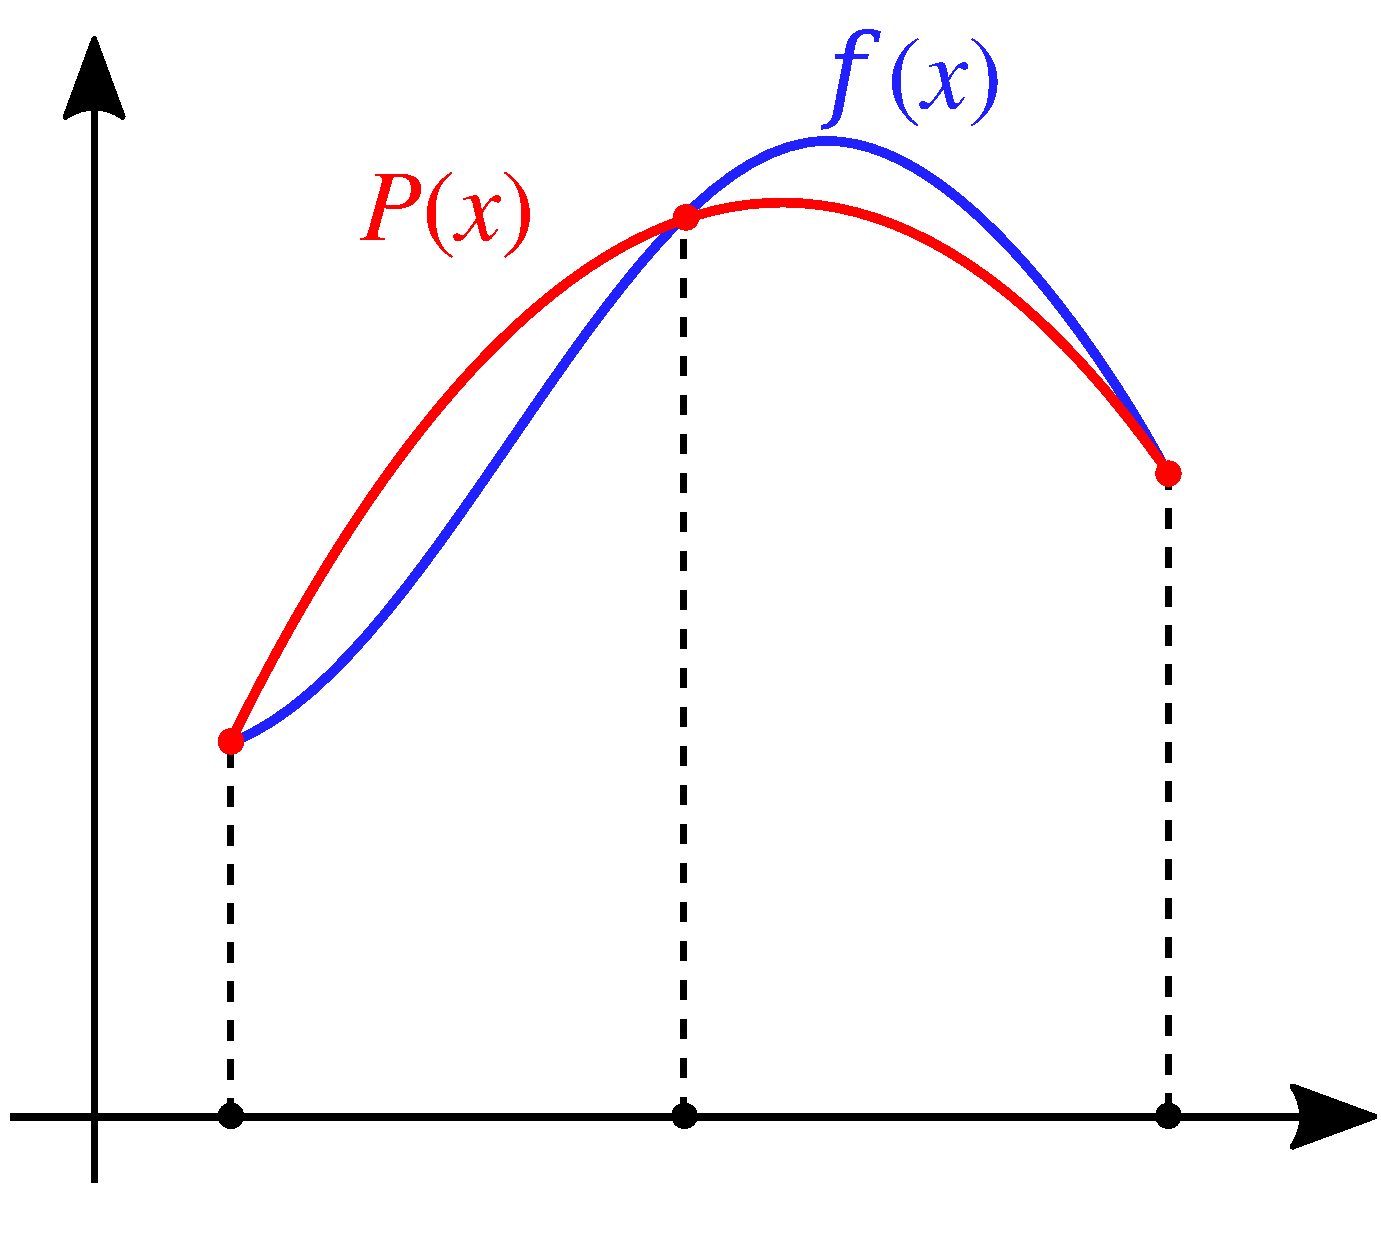
\includegraphics[width = 0.2\linewidth]{Simpson's Rule.pdf}
\caption{Approximating $f(x)$ by a parabola $P(x)$. (\href{https://bit.ly/simpsons-rule}{Image} by \href{https://commons.wikimedia.org/wiki/User:Popletibus}{Popletibus} licensed under \href{https://creativecommons.org/licenses/by-sa/4.0/}{CC BY-SA 4.0})}
\label{fig:simpsonsrule}
\end{figure}
\begin{equation}{\label{eq:cs}}
{ \int _{a}^{b}f(x)\,dx\approx {\frac {b-a}{6}}\left[f(a)+4f\left({\frac {a+b}{2}}\right)+f(b)\right]}
\end{equation}
If \ref{eq:cs} is applied to $n$ equally spaced subdivisions in $[a, b]$, we get the \emph{composite Simpson's rule} \ref{eq:csr}.
\begin{equation}{\label{eq:csr}}
	 \int _{a}^{b}f(x)\,dx\approx {\frac {\Delta x}{3}}\left(f(x_{0})+4f(x_{1})+2f(x_{2})+4f(x_{3})+2f(x_{4})+\cdots +4f(x_{n-1})+f(x_{n})\right)
\end{equation}
where each of the $n+1$ ordinates is given by $x_i = a+i\Delta x$ for $i = 0,1,\ldots,n$ and $\Delta x = \mfrac{b-a}{n}$
\begin{note}
	Simpson's rule can only be applied when an odd number of ordinates is chosen.
\end{note}
\textbf{Problem Statement:}\\
\begin{equation}{\label{eq:pi_integral}}
{ \pi={22 \over 7} - \int _{0}^{1}{x^{4}(1-x)^{4} \over 1+x^{2}}\,dx } 
\end{equation}
% $\pi$ can be approximated using \ref{eq:pi_integral}\\
% \begin{equation*}{\label{eq:simp}}
% 	x = \int_{0.5}^{1}\frac{\sin\theta}{\theta}\d\theta
% \end{equation*}
Calculate $\pi_n$ (approximate \ref{eq:pi_integral} using $n$ ordinates) for all test cases (accurate till 15 decimal places).% See Starter code (below) for more details.
\begin{testcases}
	{$t$ \hfill(number of test cases, an integer)\\$n_1\ n_2\ \ldots\ n_t$ \hfill($t$ space seperated integers for each testcase)}
	{$\pi_{n_i}$ \hfill(each test case on a newline, accurate till 15 decimal places)}
	{$0 < n_i < 500$ and $n_i$ is odd}
	{10\\3 5 7 11 15 31 57 99 163 441}
	{3.140773809523810\\3.141684884891457\\3.141601987350571\\3.141593090129691\\3.141592711563659\\3.141592654188570\\3.141592653603947\\3.141592653590286\\3.141592653589817\\3.141592653589793}
	{https://github.com/paramrathour/CS-101/tree/main/Starter Codes/Simpson's Rule.cpp}
\end{testcases}
\begin{funvideo}
\href{https://youtu.be/851U557j6HE}{Researchers thought this was a bug (Borwein integrals) -- 3Blue1Brown}
\end{funvideo}
}
\end{document}